\section{cnn}
\begin{frame}{Conv-SDNN预测模型——引言}
    基于卷积结构的SDNN预测模型:随机映射CNN模型
    \begin{itemize}
        \item 随机映射CNN在图像生成任务(纹理生成、风格迁移)上具有不亚于梯度下降训练CNN的表现
    \end{itemize}
    \vspace*{-0.5em}
    \begin{figure}
        \centering
        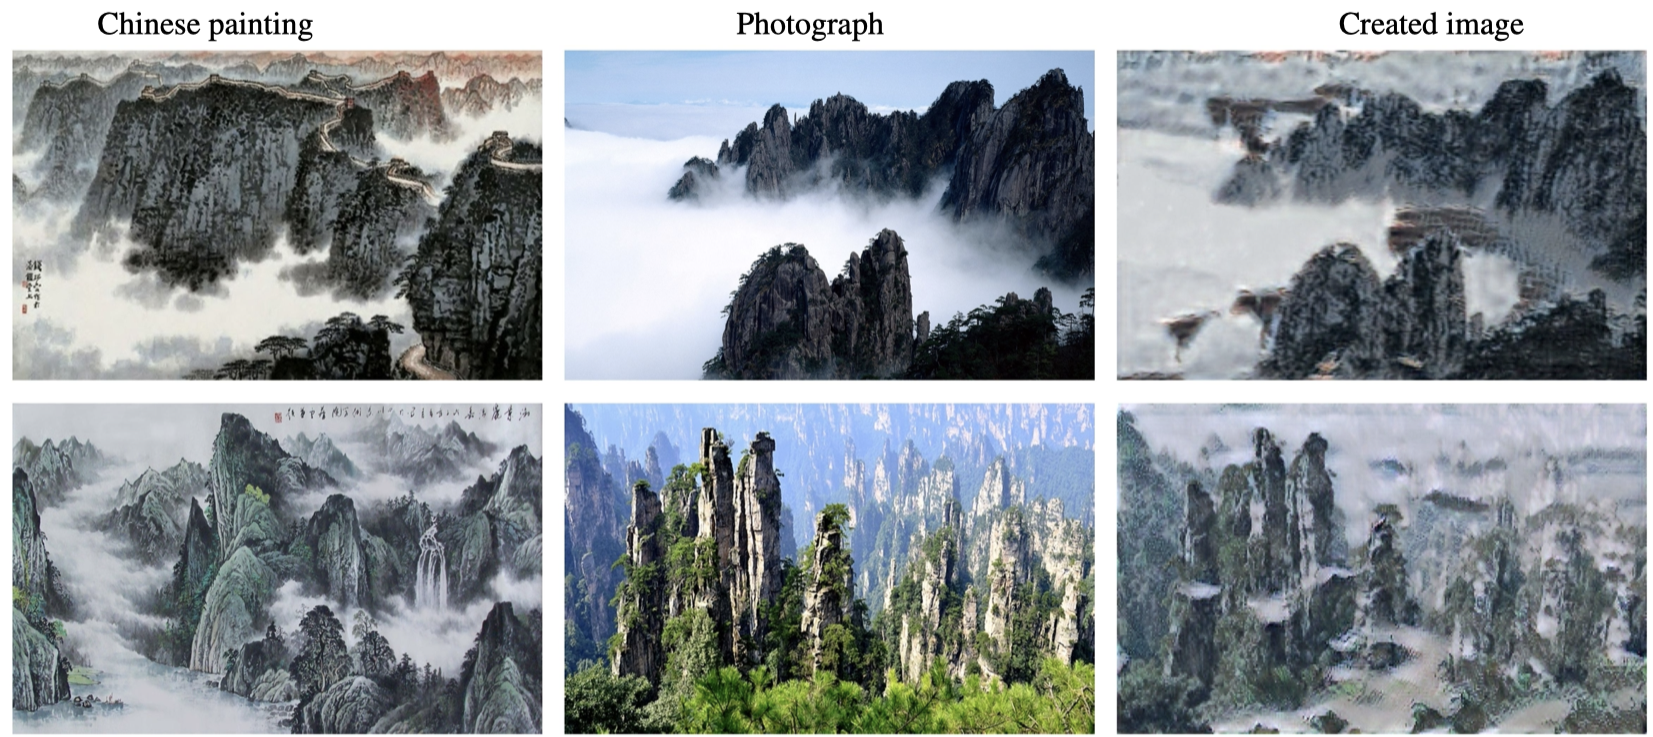
\includegraphics[width=0.9\linewidth]{float/ch.cnn/ranVGG.png}
    \end{figure}
\end{frame}

\begin{frame}{Conv-SDNN预测模型——引言}
    随机映射CNN模型研究:
    \begin{itemize}
        \item 一维随机映射CNN在一些人工时间序列预测数据集上展现出比MLP模型更好的拟合性能(Yu et al. 2019)
    \end{itemize}
    \vspace*{-0.5em}
    \begin{figure}
        \centering
        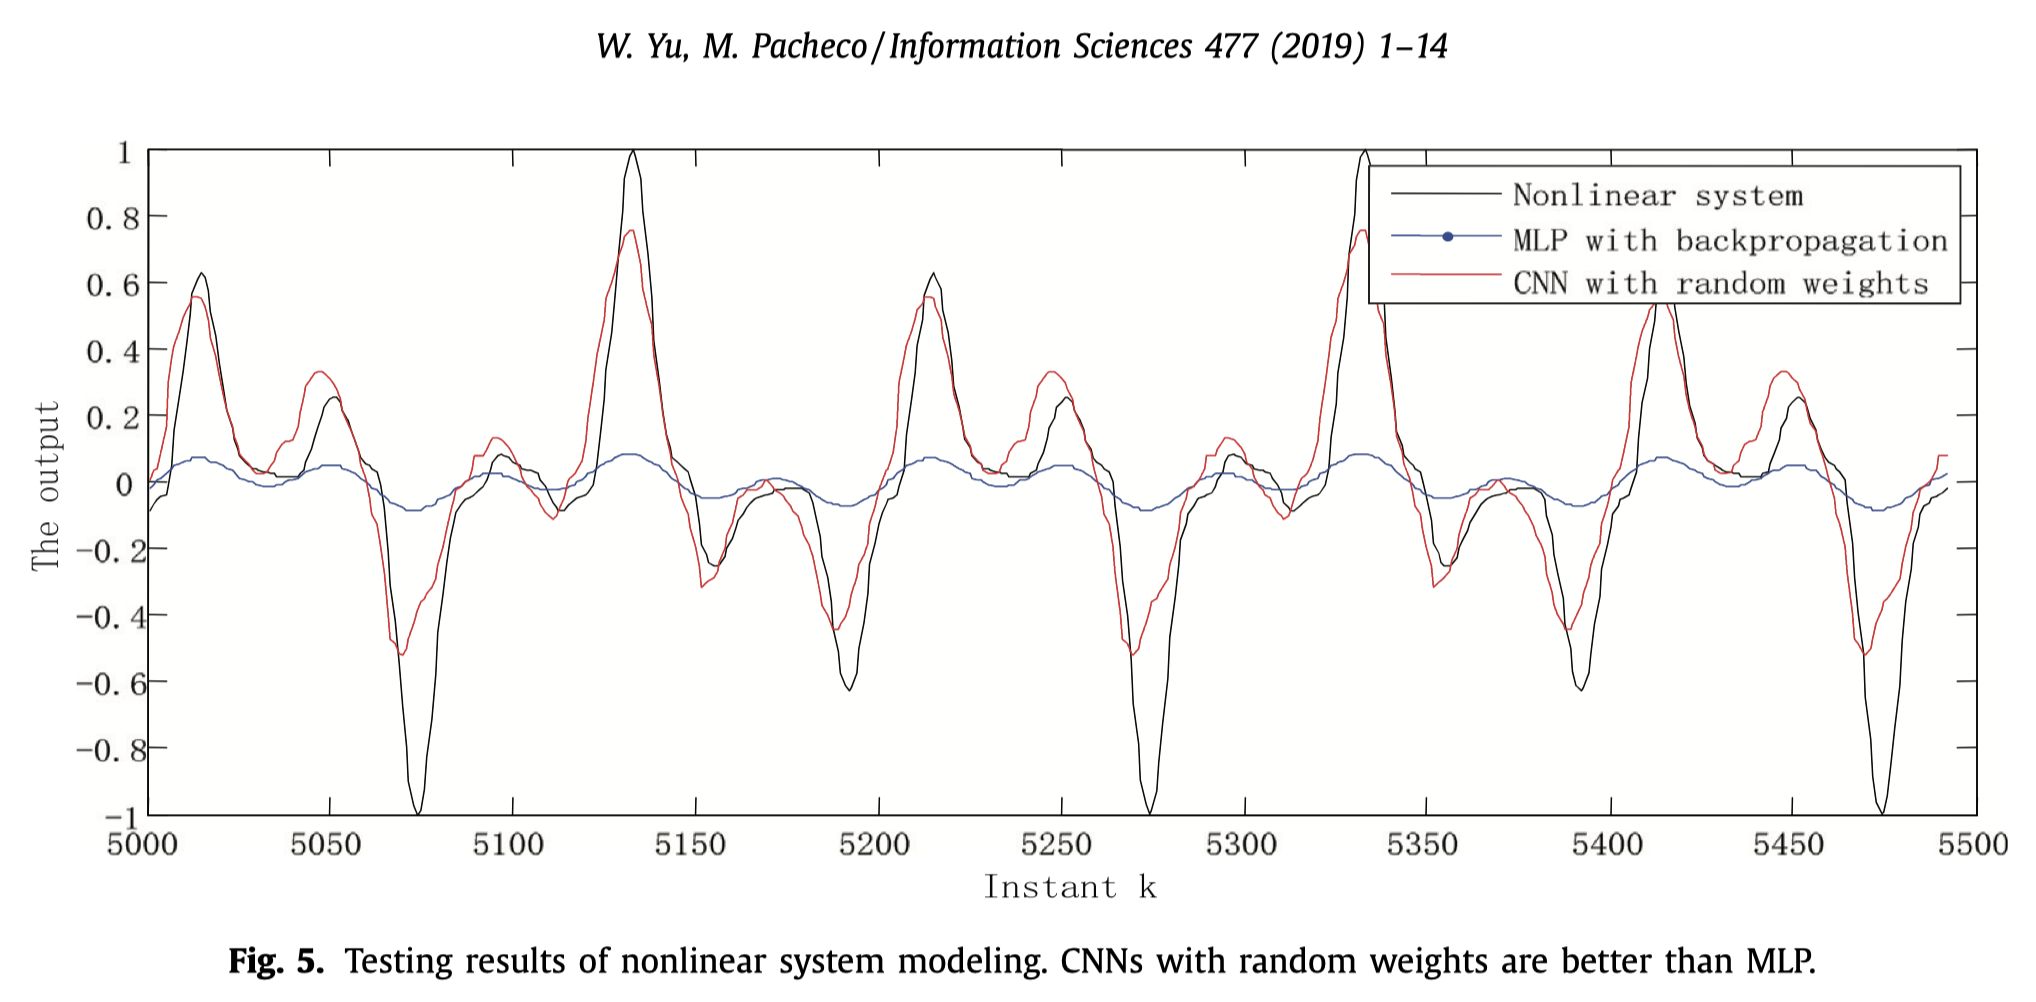
\includegraphics[width=0.9\linewidth]{float/ch.cnn/yu.png}
    \end{figure}
\end{frame}

\begin{frame}{Conv-SDNN预测模型——引言}
    随机映射CNN模型研究归纳:
    \begin{itemize}
        \item 既有研究较少,已有随机映射CNN模型性能有限,亟待新的随机映射CNN预测模型及其构造技术
    \end{itemize}

    \vspace*{0.5em}
    本章贡献:
    \begin{itemize}
        \item 基于误差反馈随机映射的随机映射CNN预测模型构造方法
              \begin{itemize}
                  \item 通过递归生成随机映射卷积核的方式提高了模型构造效率
                  \item 借助基于误差反馈策略保证了所构造模型的理论收敛性
              \end{itemize}
        \item 引入贪心算法解决模型构造中随机映射卷积核的选择问题
              \begin{itemize}
                  \item 自适应的在单卷积层内具备不同卷积宽度的卷积核
              \end{itemize}
        \item 与梯度下降深度学习模型和传统随机映射模型相比,ESM-CNN具有优秀的预测性能与建模效率
    \end{itemize}

\end{frame}


\begin{frame}{Conv-SDNN预测模型——CNN预测模型}


    \begin{figure}[!t]
        % \newlength{\twosubht}
        % \newsavebox{\twosubbox}
        \centering
        % \begin{minipage}{0.8\textwidth}
        %     \includegraphics[width = \textwidth]{float/ch.eto/esc.png}
        %     \caption*{回声状态卷积(ESC)结构}
        % \end{minipage}
        \begin{minipage}{0.8\textwidth}
            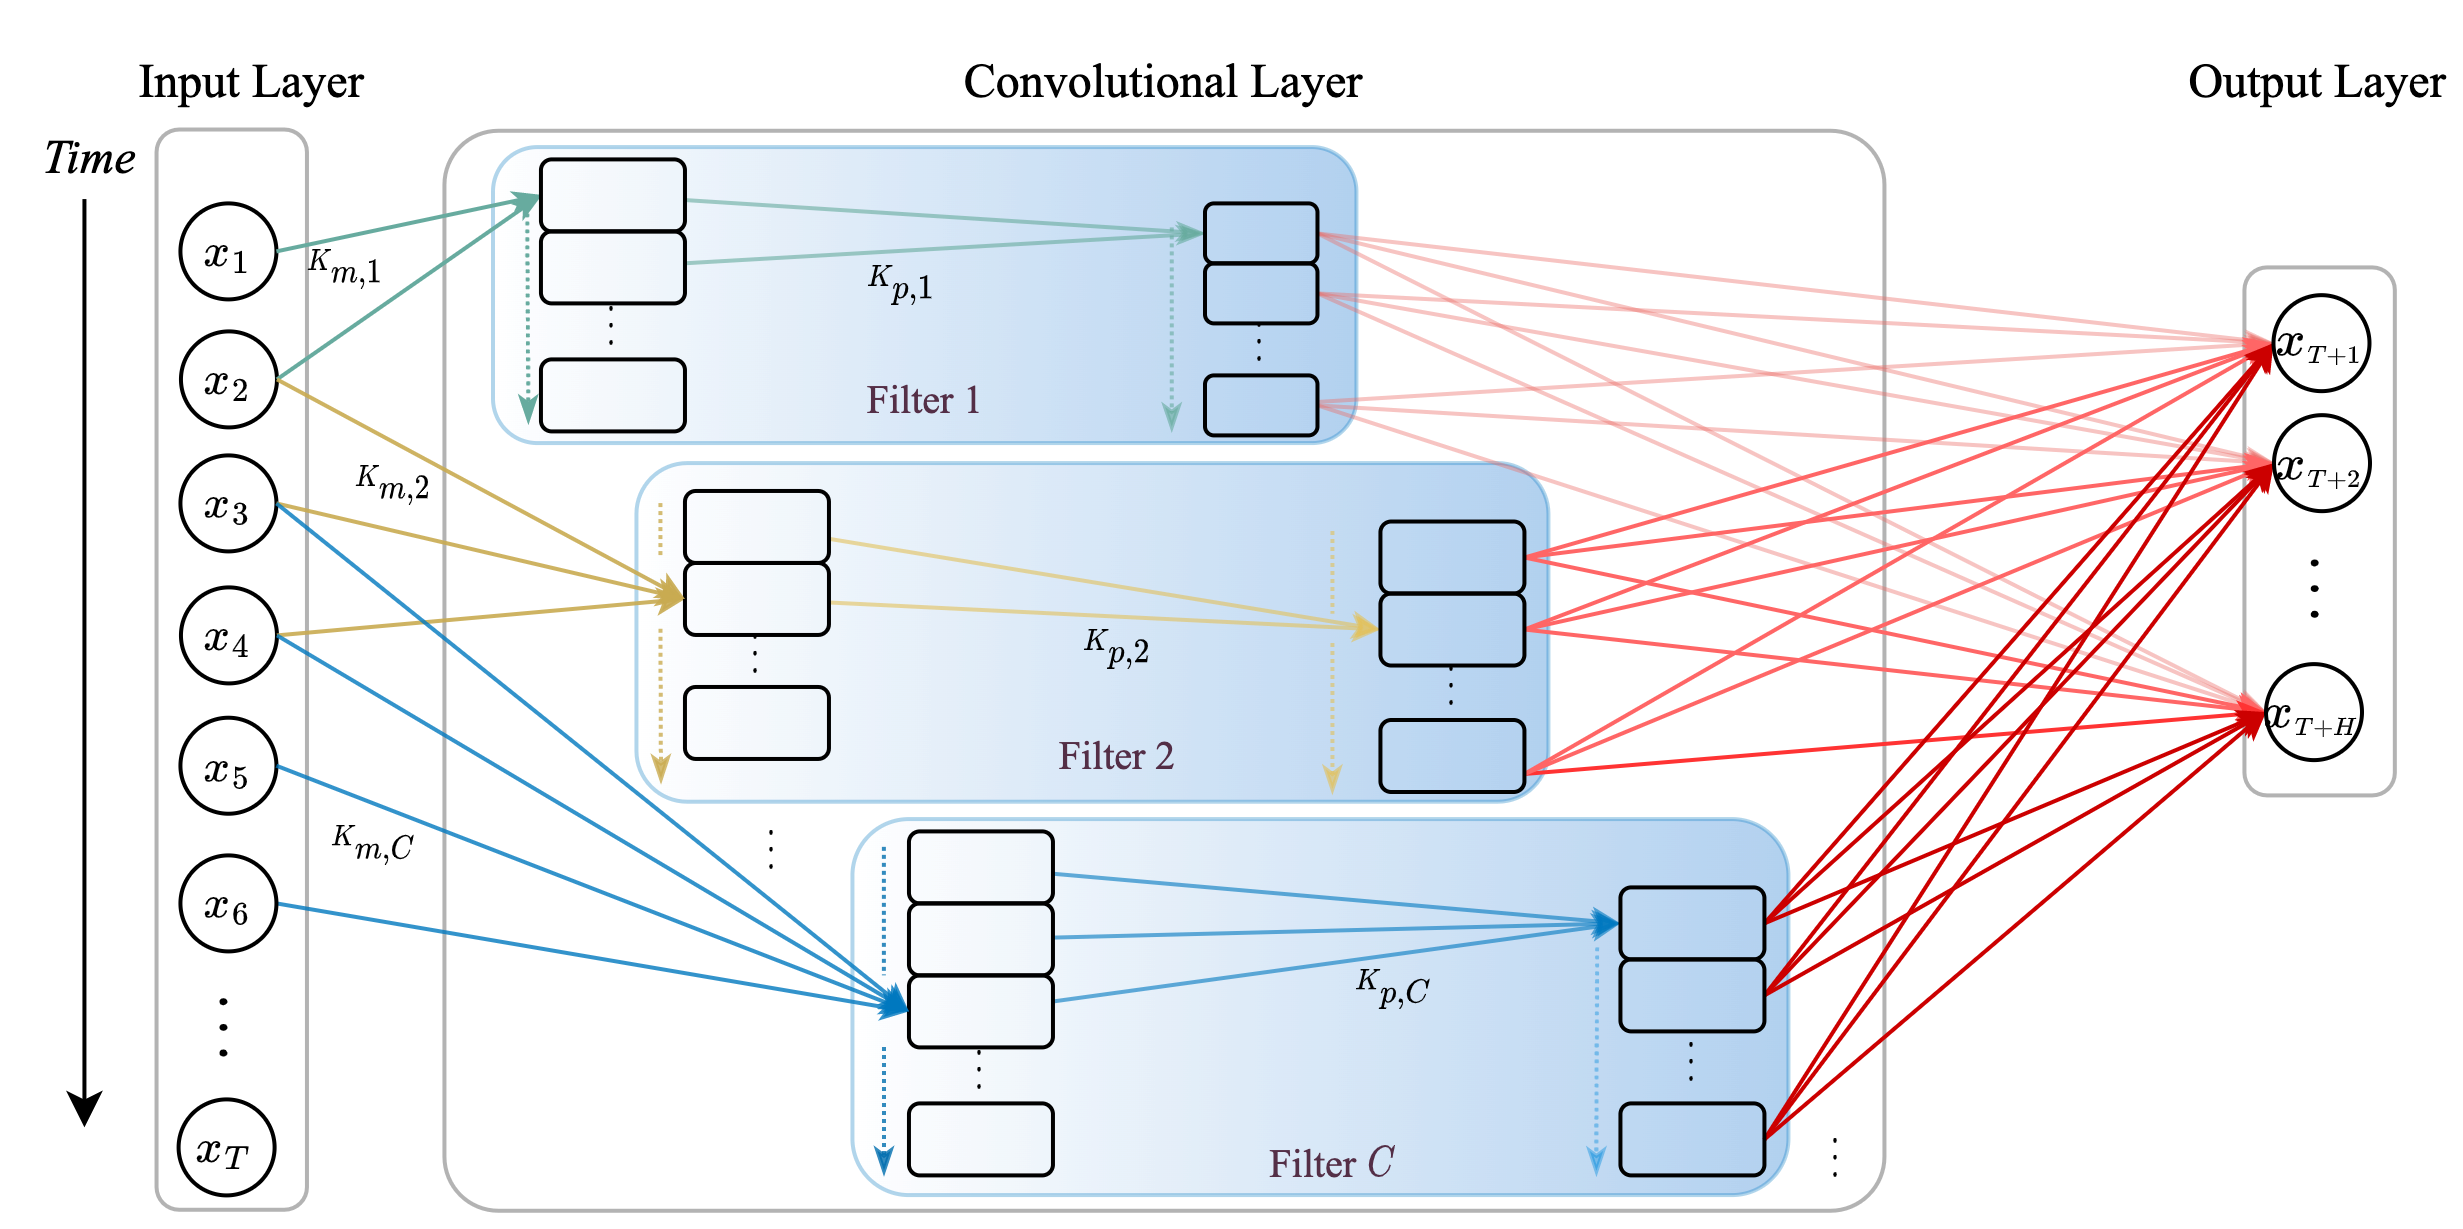
\includegraphics[width = \textwidth]{float/ch.cnn/esm-cnn.png}
            \caption*{CNN结构}
        \end{minipage}    
        % \caption{\label{fig:archMix} 基于循环神经网络与卷积神经网络的混合神经网络结构示例.}
    \end{figure}



\end{frame}

\begin{frame}
    \frametitle{Conv-SDNN预测模型——误差反馈随机映射构造方法}
    \begin{itemize}
        \item 过在单卷积层内递归增长添加固定随机初始化权重卷积核的方式构造CNN隐藏结构
        \item 利用误差反馈闭式计算新增卷积核所对应的输出权重参数
    \end{itemize}

    对于一个已具有$C$个卷积核的单卷积层ESM-CNN
    \begin{equation*}
        f_C= \sum^C_{j=1}\sum^{T-K+2}_{i=0} \beta_j^i p_j^i
    \end{equation*}

    当前预测误差为:
    \begin{equation*}
        e_C = y - f_C = [e_C^1,\ldots, e_C^H].
    \end{equation*}

    新增卷积核所对应的全连接输出层权重将基于当前模型的预测误差$e_C$反馈,通过OLM加以求解:

    \vspace{-1.5em}
    \begin{equation*}
        \left[\beta_{{C+1}}^0, \ldots, \beta_{{C+1}}^{T-K+2} \right]=\argmin _{\beta}\|e_C -\sum_{i=0}^{T-K+2} \beta_{C+1}^i p_{C+1}^i \|.
    \end{equation*}
\end{frame}

\begin{frame}
    \frametitle{Conv-SDNN预测模型——拟合收敛性}

    定义ESM-CNN的预测误差中间项为:$\tilde{e}_{C+1}^{\, 0}, \ldots, \tilde{e}_{C+1}^{\, T-K+2} $,新增卷积核所对应的全连接输出层权重中间项为:$\tilde{\beta}_{C+1}^{\, 0}, \ldots, \tilde{\beta}_{C+1}^{\, T-K+2}$,中间项之间的计算关系为:
    \begin{alignat*}{2}
         & \tilde{e}_{C+1}^{\, i+1}       & = & \mspace{18mu} \tilde{e}_{C+1}^{\, i}-\tilde{\beta}_{C+1}^{\, i+1} p_{C+1}^{i+1}, \quad i = 0,\ldots,T-K+1,                                        \\
        \shortintertext{其中,}
         & \tilde{\beta}_{C+1}^{\, i+1}   & = & \mspace{18mu} [\tilde{\beta}_{C+1}^{\, i+1,1}, \ldots,\tilde{\beta}_{C+1}^{\, i+1,h},\ldots, \tilde{\beta}_{C+1}^{\, i+1,H}],                     \\
         & \tilde{\beta}_{C+1}^{\, i+1,h} & = & \mspace{18mu} \left\langle \tilde{e}_{C+1}^{\, i,h}, p_{C+1}^{\, i+1}\right\rangle /\left\|p_{C+1}^{\, i+1}\right\|^{2} , \quad h= 1, \ldots, H .
    \end{alignat*}
    可证:
    \vspace{-1em}
    \begin{align*}
            & \|\tilde{e}_{C+1}^{\, i+1}\|^2-\|\tilde{e}_{C+1}^{\, i}\|^2 \\
        ={} & \sum_{h=1}^{H}
        \left(
        \langle \tilde{e}_{C+1}^{\, i,h}-\tilde{\beta}_{C+1}^{\, i+1,h} p_{C+1}^{i+1}
        ,
        \tilde{e}_{C+1}^{\, i,h}-\tilde{\beta}_{C+1}^{\, i+1,h} p_{C+1}^{i+1} \rangle
        -
        \langle \tilde{e}_{C+1}^{\, i,h}, \tilde{e}_{C+1}^{\, i,h} \rangle
        \right)                                                           \\
        ={} & \sum_{h=1}^{H}
        \left(
        - {\langle \tilde{e}_{C+1}^{\, i,h}, p_{C+1}^{\, i+1} \rangle}^2 / \left\|p_{C+1}^{\, i+1}\right\|^{2}
        \right)      \leq 0
    \end{align*}
\end{frame}

\begin{frame}
    \frametitle{Conv-SDNN预测模型——拟合收敛性}

    该性质在$\left\|\tilde{e}_{C+1}^{\, 0}\right\|^{2}$与$\left\|e_{C}\right\|^{2}$间仍然保持,
    因此,ESM-CNN的预测误差收敛性如下:
    $$
        \|e_{C+1}\|^2  \; \leq \|\tilde{e}_{C+1}^{\, T-K+2}\|^2 \; \leq \|\tilde{e}_{C+1}^{\,0}\|^2 \; \leq \|{e}_{C}\|^2 .
    $$

    方法优势:
    \begin{itemize}
        \item 迭代局部更新输出层权重的方式具有更小的计算开销,这种低开销优势会随隐藏层结构的增大同时扩大
        \item 随着卷积层中递归新增卷积核的不断加入,链接至输出层的池化特征图向量维度会同时倍数增大,与预测目标维度相比过大的特征维度会导致闭式求解算法的病态问题(Ill-posed problem)
        \item 基于误差反馈递归更新输出权重构造的预测模型能在神经网络隐藏构造的过程中不断弥补上步预测误差,同时,这种历史输出权重保持固定的方式在一定程度上承担了正则化的作用,从而增强了所构造模型的性能稳定性
    \end{itemize}
\end{frame}

\begin{frame}
    \frametitle{Conv-SDNN预测模型——卷积核选择方法}

    针对ESM-CNN预测模型构造中的卷积核选择问题,本章节提出了一种基于贪心算法的卷积核选择方法,使得ESM-CNN具有在单卷积层中同时具备不同宽度的卷积核结构,以此增强模型对于不同尺度时间序列特征的学习建模能力。

    本节提出了一种卷积核评分$\Delta_{{C+1, s}}$,计算如下:
    \begin{align*}
        \Delta_{{C+1},s} & = \| e_{C+1,s} \|^2 - \| e_{C} \|^2 \notag                                                                        \\
        {}               & = \|\ e_C -\sum_{i=0}^{T-K^{\prime}+2} \beta_{C+1, s}^i p_{C+1, s}^i \|^2 -  \| e_{C} \|^2 \label{eq:filterScore}
    \end{align*}


    基于所提的卷积核评分,实现最好预测效果提升的备选卷积核$p_{C+1}^{*}$将被选出作为新增卷积核正式加入当前神经网络结构,该过程可被表述为:
    \begin{equation*}\label{eq:scselection}
        p_{C+1}^{*} = \argmax\limits_{p_{{C+1},s}} \{ \Delta_{{C+1},s}, s = 1,\ldots,S \}.
    \end{equation*}

\end{frame}

\begin{frame}
    \frametitle{Conv-SDNN预测模型——实验设计}

    \begin{table}[!t]
    \centering
    \caption{数据集信息 \label{tab:app_data}}
    \begin{tabularx}{\textwidth}{lccccY}
    % \caption{数据集信息 \label{tab:app_data}}\\
    \toprule
    数据集名称      & 平稳性 & 趋势性 & 季节性 &  起始截止日期  & 数据集大小 \\ \midrule
    AR1          & \xmark      & 0.97      & 0.09        & -                           & 500         \\
    BTC          & \xmark      & 0.99      & 0.66        & 05/25/2020 $\sim$ 03/20/2021 & 2181        \\
    ILI          & \cmark      & 0.51      & 0.61        & 01/15/2010 $\sim$ 04/15/2020 & 535         \\
    BRENT-weekly & \xmark      & 0.97      & 0.07        & 05/15/1987 $\sim$ 04/30/2021 & 1773        \\
    BRENT-daily  & \xmark      & 0.97      & 0.06        & 05/20/1987 $\sim$ 05/03/2021 & 8620        \\
    WTI-weekly   & \xmark      & 0.96      & 0.08        & 01/03/1986 $\sim$ 04/30/2021 & 1844        \\
    WTI-daily    & \xmark      & 0.96      & 0.07        & 01/02/1986 $\sim$ 05/03/2021 & 8904        \\
    S\&P 500           & \xmark      & 0.99      & 0.40        & 12/31/2009 $\sim$ 11/15/2017 & 1984        \\
    NASDAQ       & \xmark      & 0.99      & 0.27        & 12/31/2009 $\sim$ 11/15/2017 & 1984        \\
    DJI          & \xmark      & 0.99      & 0.40        & 12/31/2009 $\sim$ 11/15/2017 & 1984        \\
    NYSE         & \xmark      & 0.98      & 0.45        & 12/31/2009 $\sim$ 11/15/2017 & 1984        \\ \bottomrule
    \end{tabularx}
    \end{table}

\end{frame}

\begin{frame}
    \frametitle{Conv-SDNN预测模型——实验设计}

    \begin{figure}
        \begin{minipage}[t]{0.5\textwidth}
            对比模型:
            \begin{itemize}
                \item 统计预测模型
                      \begin{itemize}
                          \item Naive、ARIMA、Holt’s Winters
                      \end{itemize}
                \item 随机映射模型
                      \begin{itemize}
                          \item RVFL、IELM、SCN
                      \end{itemize}
                \item 深度学习模型
                      \begin{itemize}
                          \item GS-CNN、DeepAR、CLSTM
                      \end{itemize}
                \item 消融实验模型
                      \begin{itemize}
                          \item 移除卷积核选择 \\ \(\rightarrow\) ES-CNN
                          \item 移除误差反馈与卷积核选择 \\ \(\rightarrow\) Stoc-CNN
                      \end{itemize}
            \end{itemize}
        \end{minipage}
        \hfill
        \begin{minipage}[t]{0.45\textwidth}
            评价指标:
            \begin{itemize}
                \item 百分比误差
                      \begin{itemize}
                          \item MAPE、SMAPE
                      \end{itemize}
                \item 绝对值误差
                      \begin{itemize}
                          \item RMSE
                      \end{itemize}
            \end{itemize}

            \begin{equation*}
                MAPE = \frac1N \sideset{}{_{i=1}^N} \sum \abs{\frac{y_{i} - \hat  y_{i}}{y_i}}.
            \end{equation*}
            \begin{equation*}
                SMAPE = \frac1N \sideset{}{_{i=1}^N} \sum \abs{\frac{y_{i} - \hat  y_{i}}{y_i + \hat  y_{i}}}.
            \end{equation*}
            \begin{equation*}
                RMSE = \sqrt{\frac1N \sideset{}{_{i=1}^N} \sum ({y_{i} - \hat  y_{i}})^2 }.
            \end{equation*}
        \end{minipage}
    \end{figure}
\end{frame}


\begin{frame}
    \frametitle{Conv-SDNN预测模型——实验步骤}

    \begin{itemize}
        \item 数据集预处理:基于Z-score方法\footnote{https://scikit-learn.org/stable/modules/preprocessing.html\#preprocessing-scaler.}归一化至标准正太分布
        \item 数据集切分:按照0.64,0.16和0.2的比例切分为训练集、验证集和测试集
        \item 测试集评价:预测生成结果均先被还原至原有数值范围,再进行预测准确度计算
    \end{itemize}

    均对每一预测模型建模20次,对20次预测建模结果结合MAPE、SMAPE和RMSE指标计算预测准确度平均值,以综合表现预测模型预测准确性与稳定性

    本章节所有实验均基于CUDA 10.1版本的GPU加速Pytorch框架、Ubuntu 20.04系统环境、Intel 8700K CPU和Nvidia GTX 1070 GPU环境进行,以保证计算环境的一致性

    本章节的实验设置与算法代码已开源在Github平台\footnote{https://github.com/XinzeZhang/TimeSeriesForecasting-torch}

\end{frame}

\begin{frame}
    \frametitle{Conv-SDNN预测模型——实验结果}

    \begin{table}[!t]
\centering
\footnotesize
\caption{ESM-CNN及对照组模型在原油价格与股票指数数据集上的MAPE结果 \label{tab:app_mape}}
\resizebox{\textwidth}{!}{
\begin{tabular}{cccccccccccccc}
\toprule
\multirow{2}{*}{数据集} & \multirow{2}{*}{H} & \multicolumn{3}{c}{统计模型} & \multicolumn{3}{c}{梯度下降模型} & \multicolumn{3}{c}{随机映射模型} & \multicolumn{2}{c}{消融模型} & 所提模型\\ \cmidrule(l){3-5} \cmidrule(lr){6-8} \cmidrule(lr){9-11} \cmidrule(lr){12-13} \cmidrule(lr){14-14}
 && Naive & ARIMA& HWSES & GS-CNN& DeepAR& CLSTM & RVFL & IELM & SCN & Stoc-CNN & ES-CNN& ESM-CNN \\ \cmidrule(l){1-14}
\multirowcell{3}{BRENT-\\weekly} & 1& 5.02e-01& 1.09e-01 & 1.17e-01 & 1.60e-01 & \bf{4.37e-02} & 8.25e-02& 5.88e-02 & 1.57e-01 & 5.74e-02& 1.93e+00 & 4.57e-02& \bf{3.97e-02}\s \\\cmidrule(l){3-14}
 & 4& 4.97e-01& 2.13e-01 & 2.37e-01 & 1.78e-01 & 9.32e-02& 1.15e-01& 1.19e-01 & 1.73e-01 & 8.67e-02& 2.87e+00 & \bf{7.78e-02} & \bf{7.49e-02}\s \\\cmidrule(l){3-14}
 & 8& 5.10e-01& 3.26e-01 & 3.69e-01 & 1.82e-01 & 1.77e-01& 1.85e-01& 1.81e-01 & 2.12e-01 & 1.43e-01& 3.70e+00 & \bf{1.14e-01} & \bf{1.11e-01}\s \\\cmidrule(l){2-14}
\multirowcell{3}{BRENT-\\daily} & 1& 4.80e-01& 8.47e-02 & 8.92e-02 & 7.84e-02 & \bf{1.93e-02}\s & 3.51e-02& 2.14e-02 & 1.36e-01 & 2.01e-02& 5.06e-02 & 2.02e-02& \bf{1.99e-02} \\\cmidrule(l){3-14}
 & 5& 4.82e-01& 2.26e-01 & 2.45e-01 & 9.37e-02 & 3.48e-02& 4.44e-02& 3.92e-02 & 1.42e-01 & 3.50e-02& 8.78e-02 & \bf{3.42e-02} & \bf{3.37e-02}\s \\\cmidrule(l){3-14}
 & 10 & 4.88e-01& 3.99e-01 & 4.34e-01 & 9.50e-02 & 5.18e-02& 5.50e-02& 5.51e-02 & 1.49e-01 & \bf{5.10e-02} & 1.29e-01 & 5.37e-02& \bf{4.63e-02}\s \\\cmidrule(l){2-14}
\multirowcell{3}{WTI-\\weekly}& 1& 4.71e-01& 9.99e-02 & 1.10e-01 & 2.26e-01 & \bf{5.49e-02}\s & 1.01e-01& 7.10e-02 & 2.34e-01 & 6.33e-02& 2.10e+00 & 6.27e-02& \bf{5.77e-02} \\\cmidrule(l){3-14}
 & 4& 4.78e-01& 2.06e-01 & 2.40e-01 & 2.47e-01 & 1.11e-01& 1.45e-01& 1.34e-01 & 2.53e-01 & 1.06e-01& 3.11e+00 & \bf{9.46e-02} & \bf{8.64e-02}\s \\\cmidrule(l){3-14}
 & 8& 5.11e-01& 3.18e-01 & 3.71e-01 & 2.46e-01 & 1.72e-01& 2.16e-01& 2.06e-01 & 2.81e-01 & 1.35e-01& 3.70e+00 & \bf{1.32e-01} & \bf{1.24e-01}\s \\\cmidrule(l){2-14}
\multirowcell{3}{WTI-\\daily}& 1& 4.44e-01& 7.82e-02 & 8.33e-02 & 9.30e-02 & 2.11e-02& 3.62e-02& 2.15e-02 & 1.45e-01 & 2.14e-02& 7.24e-02 & \bf{2.08e-02} & \bf{2.06e-02}\s \\\cmidrule(l){3-14}
 & 5& 4.49e-01& 2.05e-01 & 2.21e-01 & 9.90e-02 & \bf{3.50e-02}\s & 4.65e-02& 4.14e-02 & 1.51e-01 & 3.67e-02& 1.22e-01 & 3.62e-02& \bf{3.57e-02} \\\cmidrule(l){3-14}
 & 10 & 4.60e-01& 3.57e-01 & 3.86e-01 & 9.96e-02 & 5.21e-02& 5.76e-02& 5.93e-02 & 1.58e-01 & \bf{5.20e-02} & 1.67e-01 & 5.99e-02& \bf{4.99e-02}\s \\\cmidrule(l){2-14}
\multirow{3}{*}{S\&P 500}& 1& 1.50e-01& \bf{5.17e-03}& 8.26e-03 & 1.92e-02 & 1.28e-02& 4.88e-02& 8.82e-03 & 3.95e-02 & 1.18e-02& 1.73e+00 & 5.33e-03& \bf{4.06e-03}\s \\\cmidrule(l){3-14}
 & 5& 1.46e-01& 7.15e-03 & 1.10e-02 & 2.03e-02 & 1.87e-02& 7.20e-02& 1.91e-02 & 5.20e-02 & 2.20e-02& 1.09e+01 & \bf{7.03e-03} & \bf{6.17e-03}\s \\\cmidrule(l){3-14}
 & 10 & 1.48e-01& 8.91e-03 & 1.32e-02 & 1.94e-02 & 7.97e-02& 5.95e-02& 2.40e-02 & 4.65e-02 & 3.46e-02& 1.43e+01 & \bf{8.71e-03} & \bf{8.03e-03}\s \\\cmidrule(l){2-14}
\multirow{3}{*}{NASDAQ}& 1& 1.77e-01& 7.16e-03 & 1.04e-02 & 2.84e-02 & 7.19e-03& 6.86e-02& 3.65e-02 & 5.78e-02 & 1.62e-02& 3.85e+01 & \bf{6.68e-03} & \bf{5.50e-03}\s \\\cmidrule(l){3-14}
 & 5& 1.73e-01& 1.03e-02 & 1.40e-02 & 3.09e-02 & 2.15e-02& 9.06e-02& 3.50e-02 & 6.12e-02 & 2.36e-02& 6.13e+01 & \bf{9.12e-03} & \bf{8.84e-03}\s \\\cmidrule(l){3-14}
 & 10 & 1.75e-01& 1.29e-02 & 1.73e-02 & 3.05e-02 & 1.53e-01& 8.47e-02& 3.52e-02 & 6.00e-02 & 4.35e-02& 6.43e+01 & \bf{1.15e-02} & \bf{1.13e-02}\s \\\cmidrule(l){2-14}
\multirow{3}{*}{DJI} & 1& 1.35e-01& 5.24e-03 & 8.14e-03 & 2.36e-02 & 1.07e-02& 4.28e-02& 1.55e-02 & 4.73e-02 & 7.57e-03& 6.20e+00 & \bf{5.06e-03} & \bf{4.09e-03}\s \\\cmidrule(l){3-14}
 & 5& 1.31e-01& 7.53e-03 & 1.10e-02 & 2.54e-02 & 6.72e-02& 6.54e-02& 1.84e-02 & 4.72e-02 & 1.93e-02& 4.73e+00 & \bf{7.10e-03} & \bf{6.71e-03}\s \\\cmidrule(l){3-14}
 & 10 & 1.33e-01& 9.55e-03 & 1.34e-02 & 2.56e-02 & 3.74e-02& 6.64e-02& 3.60e-02 & 4.70e-02 & 3.89e-02& 7.16e+00 & \bf{9.14e-03} & \bf{9.06e-03}\s \\\cmidrule(l){2-14}
\multirow{3}{*}{NYSE}& 1& 1.12e-01& 5.61e-03 & 8.91e-03 & 1.31e-02 & 9.30e-03& 1.53e-02& 6.55e-03 & 2.63e-02 & 9.61e-03& 6.68e-01 & \bf{4.58e-03} & \bf{4.52e-03}\s \\\cmidrule(l){3-14}
 & 5& 1.09e-01& 7.68e-03 & 1.19e-02 & 1.44e-02 & 1.93e-02& 2.30e-02& 1.82e-02 & 2.65e-02 & 1.31e-02& 9.32e-01 & \bf{6.77e-03} & \bf{6.69e-03}\s \\\cmidrule(l){3-14}
 & 10 & 1.10e-01& 9.24e-03 & 1.42e-02 & 1.53e-02 & 9.84e-02& 2.89e-02& 2.60e-02 & 2.69e-02 & 1.81e-02& 1.45e+00 & \bf{8.44e-03} & \bf{8.38e-03}\s \\ \bottomrule
\end{tabular}}
\end{table}

\end{frame}

\begin{frame}
    \frametitle{Conv-SDNN预测模型——预测准确度分析}

    \begin{enumerate}
        \item[1)]  作为随机映射神经网络,ESM-CNN在本章节选取的人工合成时间序列数据集与真实时间序列数据集上都保持了优秀的预测准确度,展现出ESM-CNN预测模型的良好应用性。
        \item[2)] 与Naive、ARIMA和Holt所代表的统计模型相比,ESM-CNN在本章节设置的所有预测任务和所有评价指标上都表现出更优的预测准确度,展现出ESM-CNN预测模型的良好预测性能。
        \item[3)] 与GS-CNN、DeepAR和CLSTM所代表的梯度下降训练深度学习预测模型相比,ESM-CNN在本章节设置的绝大部分预测任务和评价指标上取得了更优的预测准确度;在梯度下降训练模型取得最优结果的预测任务中,ESM-CNN预测模型也取得了差距很小的次优预测结果,展示出ESM-CNN预测模型与梯度下降训练深度学习预测模型匹敌的预测能力。
        \item[4)] 与RVFL、IELM和SCN所代表的随机映射MLP预测模型相比,ESM-CNN同样在本章节设置的所有预测任务和所有评价指标上都表现出更优的预测准确度,展示出ESM-CNN预测模型在随机映射预测模型中的预测优势。
    \end{enumerate}

\end{frame}



\begin{frame}
    \frametitle{Conv-SDNN预测模型——消融实验分析}

    \begin{enumerate}
        \item[1)] 仅单纯引入随机映射方法的Stoc-CNN预测模型在本章节选取的所有预测任务和所有评价指标上都表现出显著弱于ES-CNN与ESM-CNN的预测性能,并在多项预测任务中表现出最差的预测准确度,验证了病态问题在全局更新输出权重方式下所导致的预测性能问题。
        \item[2)] 引入误差反馈随机映射构造策略的ES-CNN预测模型与Stoc-CNN相比,取得了显著的准确度提升,并在大部分预测任务和评价指标中表现出次优的水平,展现出基于误差反馈随机映射策略构造CNN预测模型的有效性与必要性。
        \item[3)] 与ES-CNN和Stoc-CNN预测模型相比,ESM-CNN在本章节设置的所有预测任务和所有评价指标上都表现出更优的预测准确度,证明了所提卷积核选择方法在ESM-CNN预测模型构造过程中的有效性与必要性。
    \end{enumerate}

\end{frame}

\begin{frame}
    \frametitle{Conv-SDNN预测模型——收敛性分析}
    \begin{figure}[!t]
        \centering
        \begin{minipage}[b]{0.32\textwidth}
            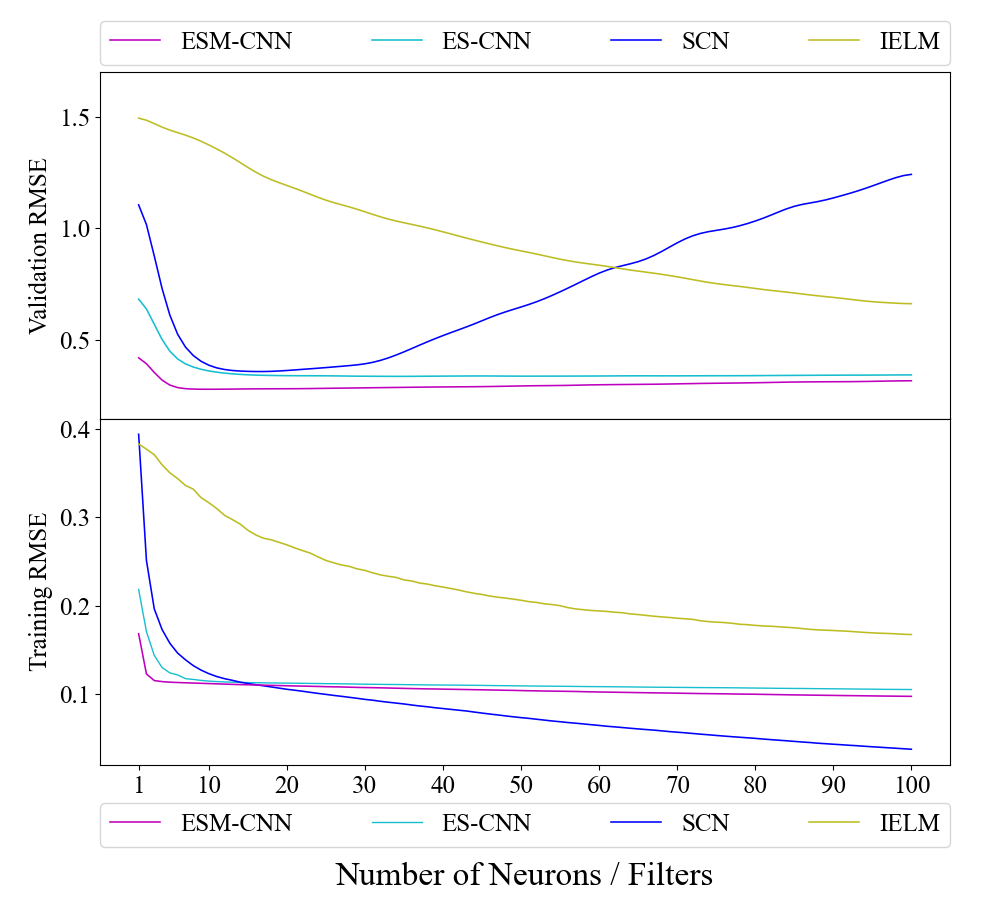
\includegraphics[width = 0.95\textwidth]{float/ch.cnn/sili_H1_revise.png}
            \subcaption{ ILI, $H = 1$ }
        \end{minipage}
        \begin{minipage}[b]{0.32\textwidth}
            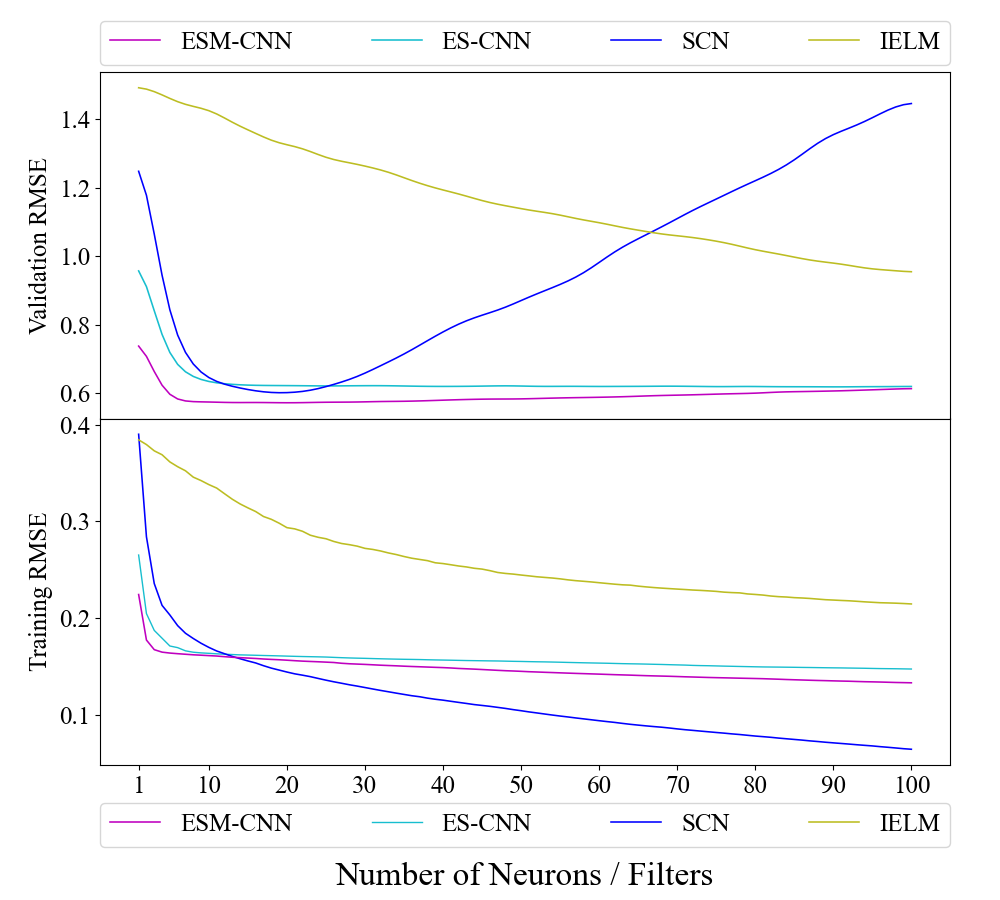
\includegraphics[width = 0.95\textwidth]{float/ch.cnn/sili_H4_revise.png}
            \subcaption{ ILI, $H = 4$ }
        \end{minipage}
        \begin{minipage}[b]{0.32\textwidth}
            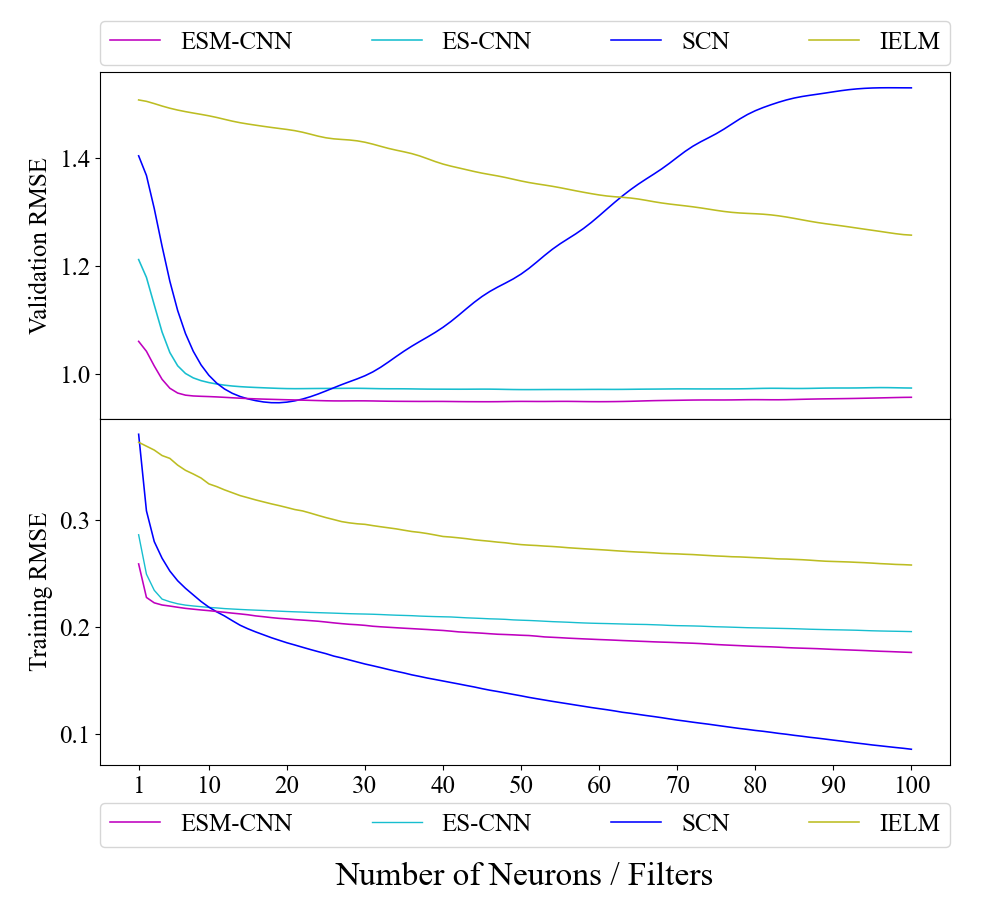
\includegraphics[width = 0.95\textwidth]{float/ch.cnn/sili_H8_revise.png}
            \subcaption{ ILI, $H = 8$ }
        \end{minipage}

        \caption*{ILI数据集上递归增长随机映射神经网络的RMSE曲线}
    \end{figure}
\end{frame}

\begin{frame}
    \frametitle{Conv-SDNN预测模型——收敛性分析}

    \begin{enumerate}
        \item[1)] 同一预测模型在不同预测时长任务上的收敛情况是一致的。
        \item[2)] 尽管SCN模型在不同预测任务的训练集RMSE上都能做出最快收敛,但SCN模型在进行真实预测建模中出现了明显的过拟合现象,而采用误差反馈策略的IELM模型并没有出现过拟合,但表现出最慢的收敛速度。这一对比结果证明了误差反馈策略解决过拟合问题的有效性,同时也指出了误差反馈策略下MLP结构的性能局限性。
        \item[3)] 基于卷积结构的ESM-CNN和ES-CNN在所有的验证集RMSE中都表现出比IELM和SCN更快且更低的收敛效果,证明了基于误差反馈随机映射构造CNN预测模型的收敛性与鲁棒性。
        \item[4)] 与ES-CNN相比,ESM-CNN具备更低的训练集RMSE曲线和测试集RMSE曲线,从收敛性角度再次验证了所提卷积核选择方法的有效性与必要性。
        \item[5)] 在ESM-CNN与ES-CNN的收敛过程中,预测性能的最大增益明显来自于构造过程的前10步,表现出ESM-CNN具备通过牺牲微小性能换来巨大效率提升的平衡策略,从而使得ESM-CNN具有更加广泛和高效的现实应用性。
    \end{enumerate}

\end{frame}

\begin{frame}
    \frametitle{Conv-SDNN预测模型——建模效率分析}
    \begin{table*}[!t]
    \centering
    \footnotesize
    \caption{神经网络模型在AR1、BTC和ILI数据集上的单次平均建模时间(s) \label{tab:time}}
    \resizebox{\textwidth}{!}{\begin{tabular}{ccrrrrrrrrr}
        \toprule
        \multirow{2}{*}{建模方法}   & \multirow{2}{*}{模型} & \multicolumn{3}{c}{AR1} & \multicolumn{3}{c}{BTC} & \multicolumn{3}{c}{ILI}                                           \\\cmidrule(lr){3-5} \cmidrule(lr){6-8}\cmidrule(lr){9-11}
                          &                         & \multicolumn{1}{c}{1} & \multicolumn{1}{c}{3} & \multicolumn{1}{c}{6} & \multicolumn{1}{c}{1} & \multicolumn{1}{c}{3} & \multicolumn{1}{c}{6} & \multicolumn{1}{c}{1} & \multicolumn{1}{c}{4} & \multicolumn{1}{c}{8} \\ \midrule        
        
\multirow{3}{*}{梯度下降} & GS-CNN                  & 74.65                 & 76.95                 & 78.55                 & 93.70                 & 96.45                 & 99.40                 & 67.05                 & 70.25                 & 73.00                 \\
                          & DeepAR                  & 225.25                & 238.95                & 257.70                & 223.75                & 251.10                & 268.65                & 256.80                & 279.10                & 275.30                \\
                          & CLSTM                   & 150.45                & 154.80                & 160.25                & 143.00                & 141.50                & 142.25                & 167.40                & 170.80                & 175.30                \\
\specialrule{0em}{1.5pt}{1.5pt}                          
\multirow{3}{*}{随机映射}   & RVFL                    & \multicolumn{1}{c}{-} & \multicolumn{1}{c}{-} & \multicolumn{1}{c}{-} & \multicolumn{1}{c}{-}  & \multicolumn{1}{c}{-}  & \multicolumn{1}{c}{-}  & \multicolumn{1}{c}{-} & \multicolumn{1}{c}{-} & \multicolumn{1}{c}{-} \\
                          & IELM                    & 2.65                  & 2.85                  & 2.80                  & 3.40                  & 3.30                  & 3.20                  & 2.55                  & 2.55                  & 2.40                  \\
                          & SCN                     & 22.85                 & 57.40                 & 107.75                & 21.10                 & 58.00                 & 111.40                & 16.10                 & 49.60                 & 90.95                 \\
\specialrule{0em}{1.5pt}{1.5pt}                          
\multirow{2}{*}{消融方法} & Stoc-CNN                & \multicolumn{1}{c}{-} & \multicolumn{1}{c}{-} & \multicolumn{1}{c}{-} & \multicolumn{1}{c}{-}  & \multicolumn{1}{c}{-}  & \multicolumn{1}{c}{-}  & \multicolumn{1}{c}{-} & \multicolumn{1}{c}{-} & \multicolumn{1}{c}{-} \\
                          & ES-CNN                  & 6.50                  & 6.40                  & 6.50                  & 6.35                  & 6.50                  & 6.45                  & 6.45                  & 6.50                  & 6.50                  \\
\specialrule{0em}{1.5pt}{1.5pt}                          
所提方法                       & ESM-CNN                 & 9.65                  & 9.65                  & 9.70                  & 7.10                  & 7.25                  & 7.25                  & 7.15                  & 7.15                  & 7.20                  \\ \bottomrule
    \end{tabular}}
\end{table*}

\end{frame}

\begin{frame}
    \frametitle{Conv-SDNN预测模型——小结}

    \textbf{(1)基于卷积结构的SDNN预测模型构造与优化方法}
    \begin{itemize}
        \item 通过代数推导证明了基于该方法所构造的预测模型具有随着卷积核的增加而单调下降的预测误差,以此保证了所提方法的收敛性,且其确定的输出权重与既有方法相比具有更小的$L_2$范数,以此提升了模型的预测稳定性;
        \item 区别于既有方法仅能用相同宽度的卷积核构造单卷积层,通过贪心选择由不同卷积核宽度组成的备选集,使得模型能够在迭代构造模型的过程中自适应确定卷积参数,其构造的单卷积层具备不同宽度的卷积核,使模型借助单卷积层具备不同尺度局部特征的学习能力;
        \item 在人工合成数据、流感阳率数据、原油价格数据和金融指数数据上的实验表明,与梯度下降训练的深度神经网络预测模型相比,基于本方法所构造的模型在具备相近甚至更优的预测准确度同时具备极高的建模效率,验证了所提方法的有效性。
    \end{itemize}

\end{frame}